\section{Introduction}
Outlining the main area you are researching. This may also include any motivation for investigation.
\section{Subject}
You can divide your Literature Review into several sections, one for each topic/area you are reviewing.
\subsection{title}
Each subject area will probably be broken down to several subsections.
\subsubsection{title}
It is generally unnecessary to go further than the subsection level, however, in rare circumstances the subsubsection command can be used. 


\begin{figure}
	\centering
	
\includegraphics[scale=0.5]{ch2/blossom}
	\caption{Test caption number}
\end{figure}

\section{Citation \& Reference}
Exercises show two there are two parts to a citation: the citation; and the reference. There are many styles and configurations of the citations and references, which the exercises will make clear. 

Essentially, to start with, we are going to keep this simple and use the plain bibliography setting. As we advance the national bibliography package can be used and this is in the exercises on citations. This setting orders all bibliography items in alphabetical order and only uses the cite command. It does have its restrictions and we will come across these and how to cope with them. The following is an example paragraph using citations and a plain bibliography and should be adequate to get us started.


The first generation of Neural Networks are generally considered as Perceptrons \cite{rosenblatt1958perceptron}. Minsky and Papert \cite{minsky1969perceptrons} wrote a critique of the perceptron which showed that it could not solve non-linear problems, typically XOR. To solve the non-linear problem Rumelhart, Hinton and Williams \cite{rumelhart1988learning} made an enormous contribution with the Back-propagation error Artificial Neural Network, ANN. This and related ANN are generally referred to as second generation and inspire many of the techniques used in machine learning. The third generation of neural networks are based on biologically-inspired neurons and are generally referred to as, ``spiking neurons''.  Oddly many third generations are based on research pre-dating to first and second generations, namely Hebbian Learning \cite{Hebb}. These spiking neurons can be built into bigger networks to solve complex problems, e.g., see \cite{huyck2013compensatory}.

\section{Example of glossary}
There are several blockchain \gls{ca1} but three of interest are: \gls{poet}, \gls{pow} and \gls{pos}.

\gls{poet} is fast and can only be used on permission blockchains. \gls{pow} is computationally expensive and can be used on permissionless blockchains, many researchers have commented that \gls{pow} is unsustainable. \gls{pos} is less computationally expensive and can be used on permissionless blockchain technology. 

\section{Summary}
Conclude on your main findings and how they are going to contribute to solving objectives.

This thesis is an outline and can be deviated from. For example, it would be completely justified to have two Literature Review Chapters, if the subject areas are unrelated and completely separate. Often new research can be considered as two subject areas merged together to form a new area, e.g., text-mining and e-discovery. This would result in two literature review chapters: i) text-mining; and ii) e-discovery. 

\begin{figure}
	\centering
	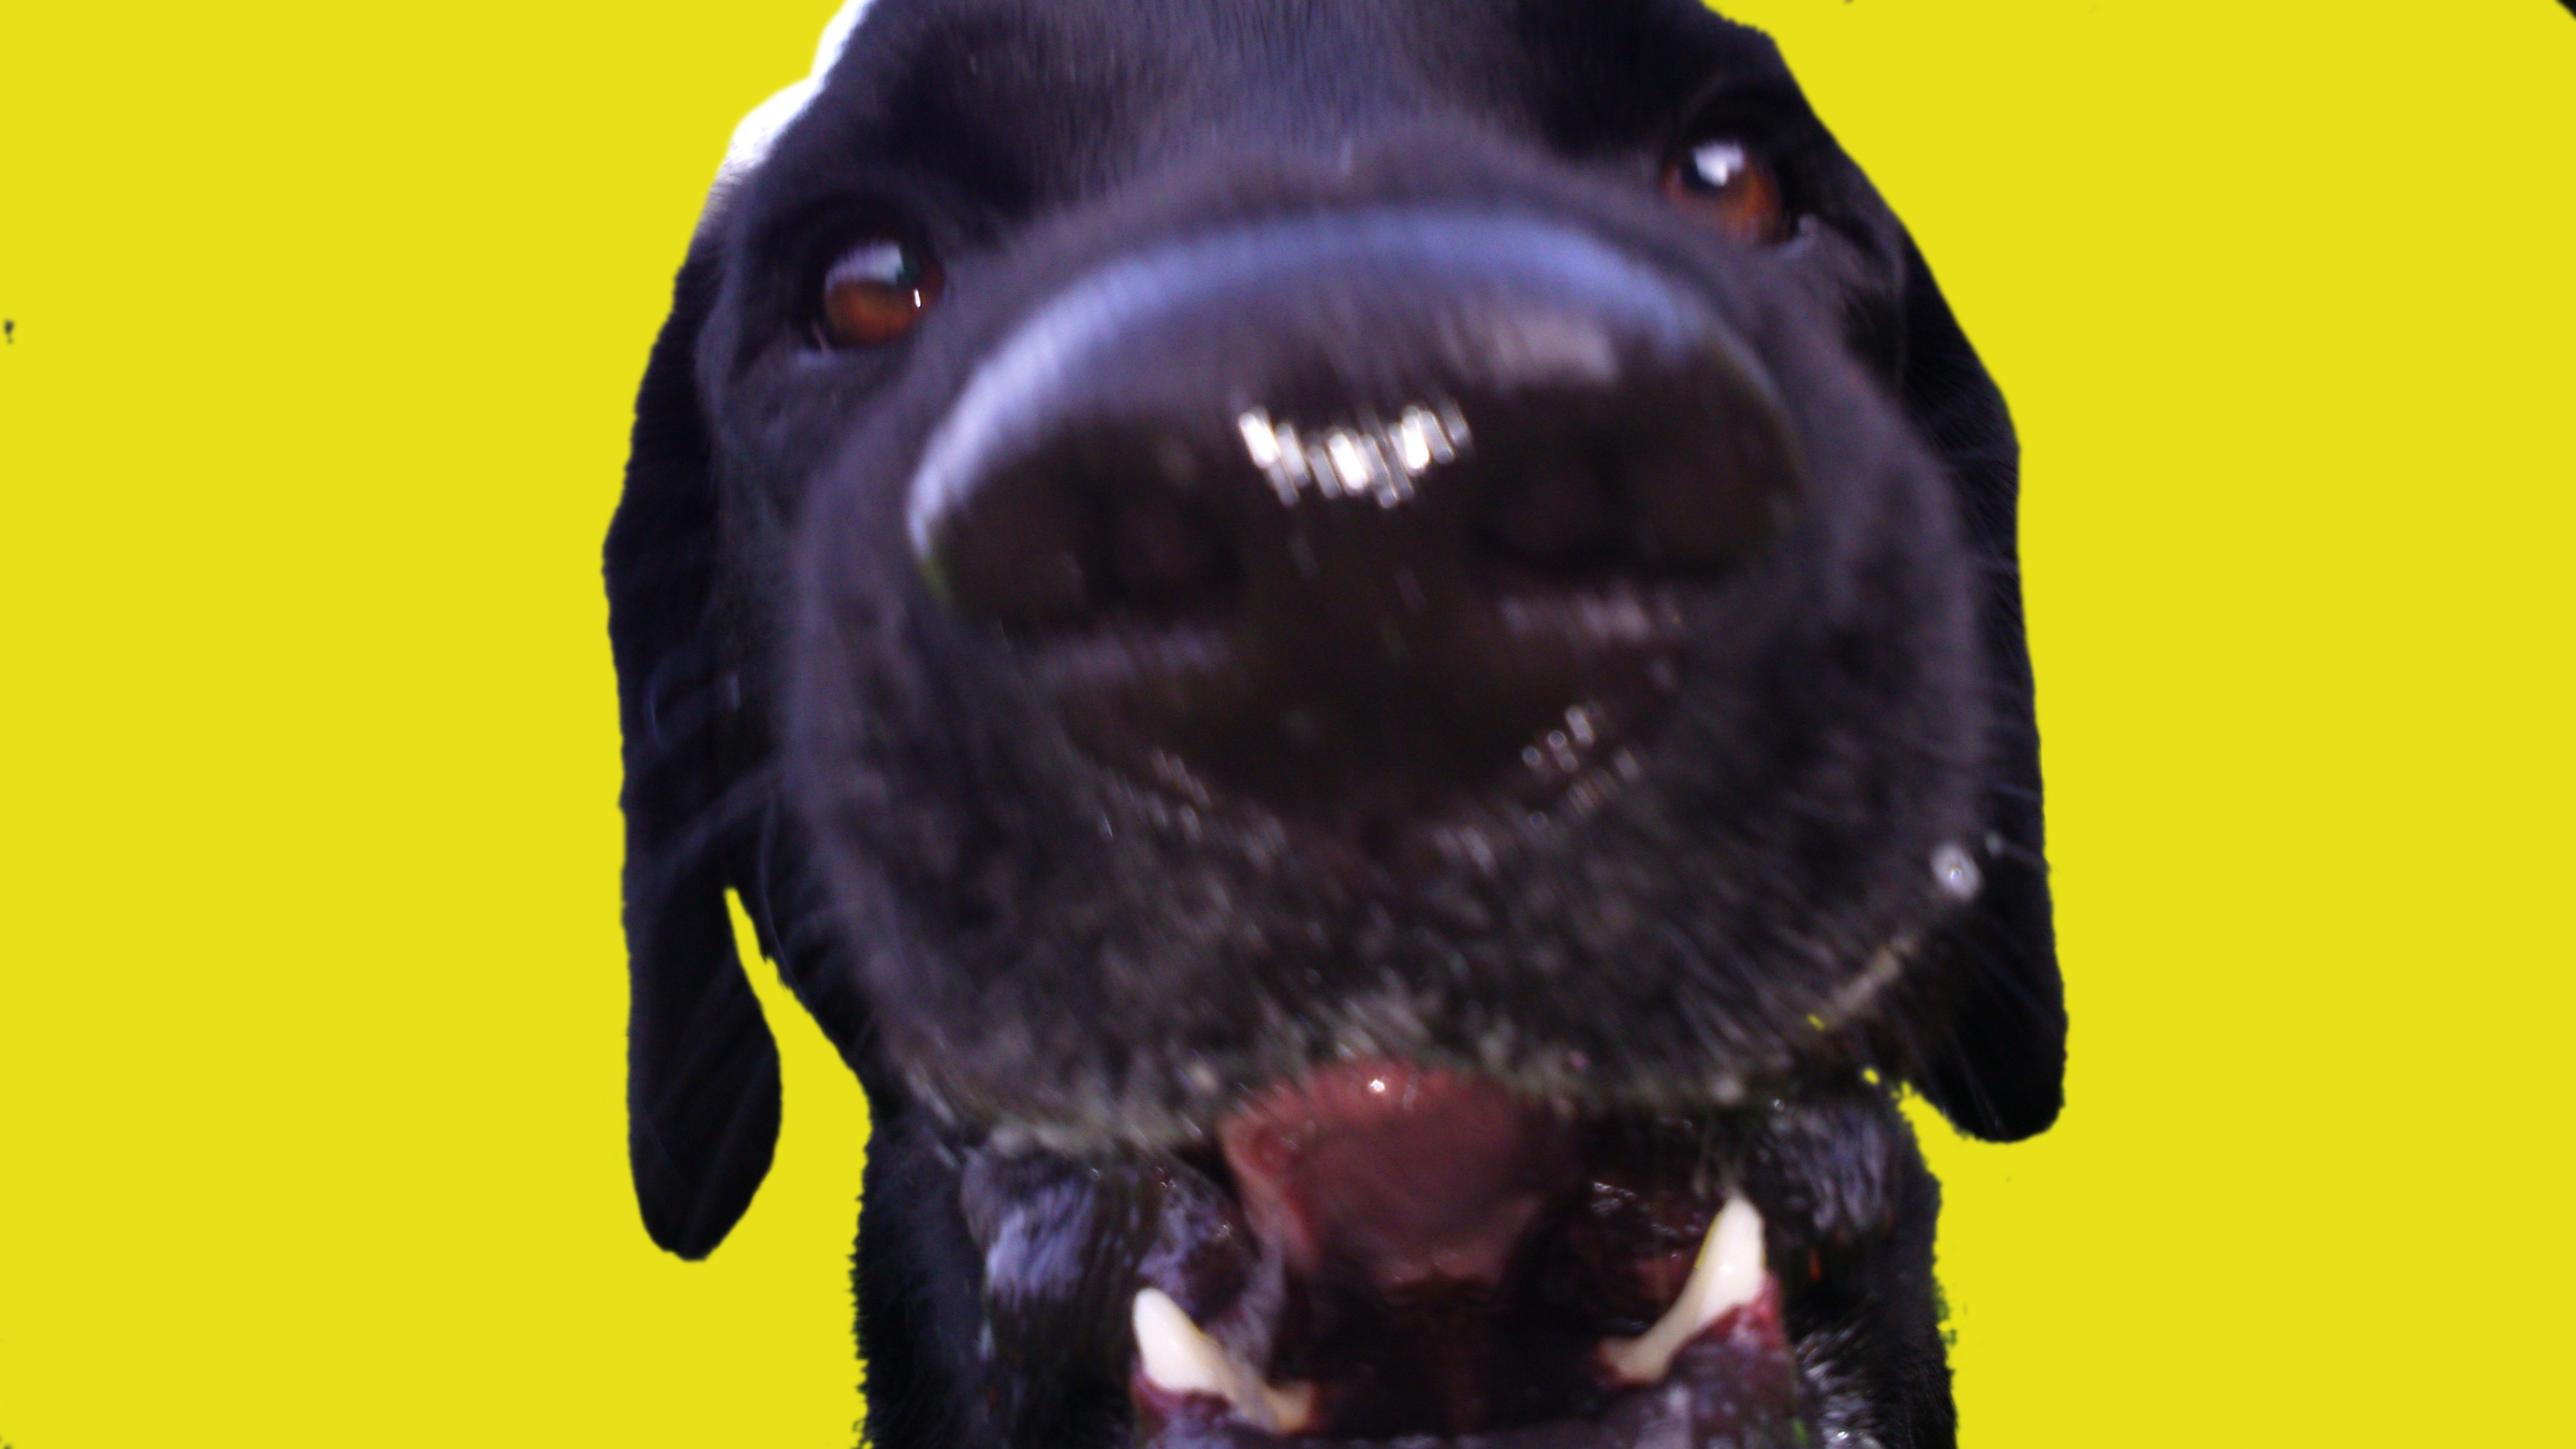
\includegraphics[scale=0.1]{ch2/awo}
	\caption{Test caption number}
\end{figure}
